\part{Solution} \label{part:solution}

\chapter{Design}

This chapter will be the occasion to detail the architecture of our solution. We will explain the technologies employed to achieve our goal, a monitoring software for Internet of Things networks. It is also in this chapter that we will justify the choices made during the development of it.

\section{Architecture}

The architecture of our solution is comprised of two parts as can be seen on Fig.\ref{fig:design}. The first part is about how the data is collected and sent. The second part consists on how the data is received and treated after reception. In the remaining of the section, strong assumptions are made that the reader is familiar with Netflow, particularly Netflow v10 or IPFIX, and also its implementation for WSN which is called TinyIPFIX. If not, explanations about those particular technologies can be found in Chap \ref{chap:monitoring_tools}. \\

\begin{figure}
	\centering
	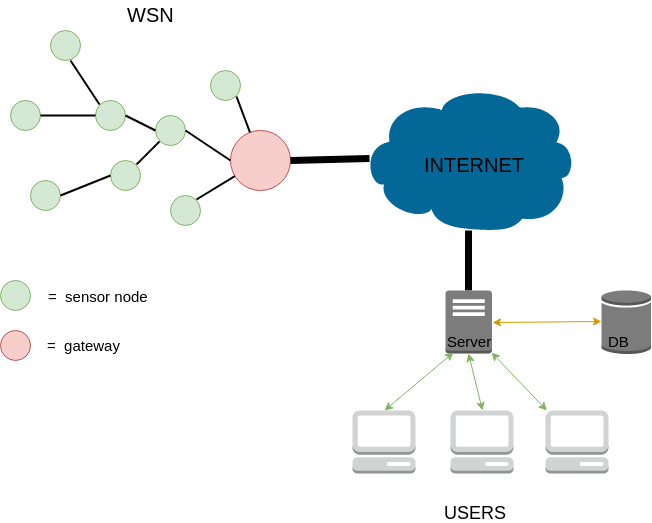
\includegraphics[width=0.8\textwidth]{res/design.png}
	\caption{Global architecture of the solution}
	\label{fig:design}
\end{figure}

The data exportation is done in a Netflow fashion. The nodes occupy the roles of exporters. Each node maintain a flow table where they register the flows that occurred during an interval of time. In our case a flow is characterized by the 4-uple: source node id, destination node id, number packets and number octets. After a certain amount of time passes, each node will construct a TinyIPFIX message based on the content of its flow table. Those messages are sent to the gateway node. The gateway node will then reformat the TinyIPFIX messages received into compliant IPFIX messages to a specific address, which will be in our case the address of a server.\\

The server which receives the IPFIX messages from the IoT network, plays two roles. One role is straightforward. It is the role of collector. Each message is collected by the server and logged in a database for further processing and analyzing. The other role, is of a web server. Multiple users can know the network status by having access to web pages served by the server.

\chapter{Alternatives}

\section{Nfsen, A Graphical Web Tool}
\todo{Ou placer, Avant/apres notre solution?}
\begin{figure}[!h]
	\centering
	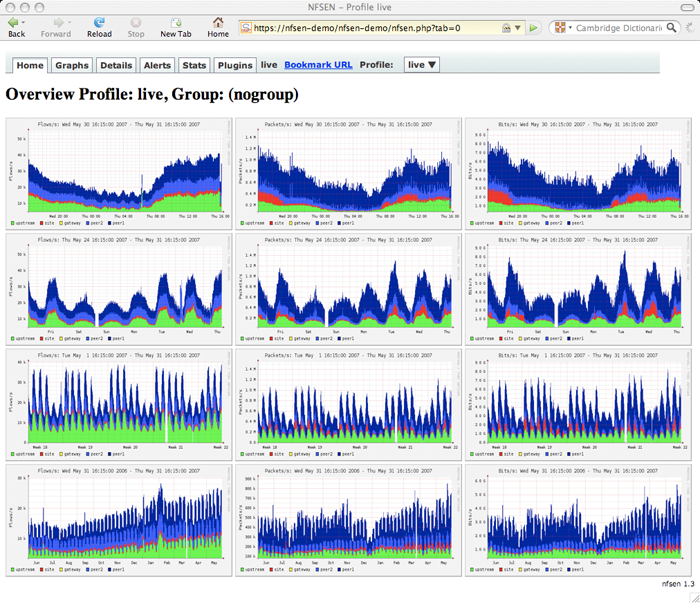
\includegraphics[width=0.8\textwidth]{res/nfsen.png}
	\caption{The Nfsen interface (source : http://nfdump.sourceforge.net/)}
	\label{fig:nfdump}
\end{figure}

The subject of our master thesis having been proposed by Professor Sadre last year and being about monitoring flows in IoT networks, the first tool that was presenting itself to us was Nfsen. Per its official website, \textit{Nfsen is a graphical web based front end for the nfdump netflow tools}. The Nfsen tool uses various graphes and charts to display the traffic of data varying with a specified time span or time interval. It works with the processing capabilities of Nfdump, a data processing tool using Netflow flows that have been retrieved from a network. Specifically, the Nfsen interface also allows to create plugins to have more ways of displaying data information. At first, it was proposed in the description of the subject of the thesis to use Nfsen along with Nfdump, particularly creating an Nfsen addon to show further information along with what Nfsen already is displaying in terms of graphical content. By plugin, one graphical content that Nfsen is lacking is the current topology of the monitored network, which can be added by making a plugin which extends the graphical tool.\\

In this section, we will explain all the underlying layers of Nfsen, from data exchanged in the monitored network to the graphical web page. We will also discuss our thought process about using Nfsen and the reasons why we have not used it in the end.\\

The first step towards monitoring is data collecting. As we explained in Chapter 3, Netflow is used for collecting flows we are interested in, according to some specific attributes such as the source and destination addresses. Once the flow are captured, they are stored and waiting to be processed. \\

(source : http://nfdump.sourceforge.net/, https://www.first.org/conference/2006/papers/haag-peter-papers.pdf)
In reality, when the structure of the Netflow data is defined, the flows are actually captured by \textit{nfcapd}, a \textit{netflow capture deamon}. With nfcapd, the flows are read from the network and the collected data is stored into files, data being split in files according to time slices. Each five minutes, nfcapd outputs a new file where data is stored, named with the current timestamp. One nfcapd process is used for each existing netflow stream that we want to capture.\\

As seen in the next figure, the next important component is \textit{nfdump}. Nfdump is a command line based tool that provides further data processing. Basically, it reads the data that was previously captured and stored by nfcapd. With Nfdump, data is aggregated and it provides further statistics about the traffic. Nfdump can either analyze the data coming from a single file, or from several of them by concatenating them before analyzing. One strength of nfdump is that it can filter out the attributes in the data that are not needed during the processing. Afterwards, the data is output either as a text file or binary data, thus being ready for further analysis. Nfdump aggregates and then creates statistics about the flows information stored, such as traffic volume sent during a timelapse. Nfdump thus acts as the backend of Nfsen.\\

\begin{figure}[!h]
	\centering
	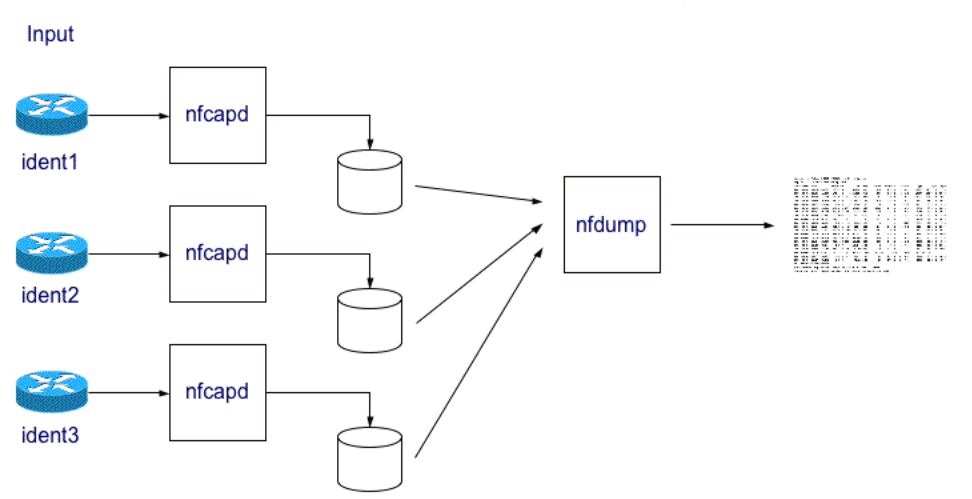
\includegraphics[width=0.8\textwidth]{res/nfdump.png}
	\caption{The Nfdump Structure (source : http://nfdump.sourceforge.net/-)}
	\label{fig:nfdump}
\end{figure}

Once the data is processed, it is displayed by Nfsen with the help of graphs. Nfsen displays the collected netflow data, either in flows, packets, or bytes. As you can see in figure \ref{fig:nfsen}, it can display various types of data, for example data sent through different protocols such as UDP, TCP, etc. It also uses time spans to select which data traffic is to be displayed (being the same time spans where nfdump did all the processing).\\

As stated earlier, Nfsen can also be extended, by creating plugins. There exist two kinds of plugins. There are the backend plugins that are written in Perl, that are created to add more functions and functionalities such as alerting conditions and data processing. On the other hand, frontend plugins are written in PHP and used to create new display fashions that the original Nfsen application would lack. In our case, we wanted to display the topology of the network under analysis, which Nfsen is not showing in its original state.
>>>>>>> 817b52e3a64792a4bcefaf15ed4452c7474ea315
